\documentclass{article}

\usepackage{geometry}
 \geometry{
 a4paper,
 total={170mm,257mm},
 left=20mm,
 top=20mm
 }
\usepackage{float}
\usepackage{graphicx}
\usepackage{indentfirst}
\usepackage{hyperref}

\graphicspath{ {./images/} }
\renewcommand*\contentsname{Daftar Isi}
\renewcommand{\figurename}{Figur}
\renewcommand{\tablename}{Tabel}

\begin{document}
	\begin{titlepage}
		\begin{center}
			
			\null
			{
				\huge \bfseries Tugas Praktikum Pengembangan Perangkat Lunak}\\
			[1cm]
			{\LARGE Project Report}\\
			
			\vspace{2cm}
			
			\begin{figure}[H]
				\centering
				
\includegraphics[width=200px]{/HitamPutih.jpg}
			\end{figure}
			
			\vspace{3cm}
			
			{\Large 
				Disusun oleh Kelompok YapaYapaHuy} {\Large :\\
				\vspace{0.5cm}
				Ardacandra Subiantoro (18/427572/PA/18532)\\
				Chrystian (18/430257/PA/18770)\\
				Juandito Batara Kuncoro (18/427582/PA/18542)\\
			}
			
			
			\vspace{2cm}
			
			{\normalsize \bfseries
				PROGRAM STUDI S1 ILMU KOMPUTER\\
				DEPARTEMEN ILMU KOMPUTER DAN ELEKTRONIKA\\
				FAKULTAS MATEMATIKA DAN ILMU PENGETAHUAN ALAM\\
				UNIVERSITAS GADJAH MADA\\
				YOGYAKARTA\\
				\vspace{0.2cm}
				2020
			}
			
		\end{center}
	\end{titlepage}

	\newpage
	\pagenumbering{arabic}
	
	\section{Background}
	\par Keadaan pandemi COVID-19 menyebabkan banyak mahasiswa kekurangan interaksi sosial sehingga mereka tidak dapat memenuhi kebutuhan sosial mereka. Hal ini dapat menyebabkan stres berlebih dan kurangnya produktivitas. Tujuan program ini adalah membantu mahasiswa yang mengalami masalah mental oleh karena keadaan pandemi dengan memberikan mereka saran dan bantuan profesional. 

	\par Untuk memenuhi kebutuhan tersebut desain perangkat lunak harus memiliki tingkat aksesibilitas yang tinggi untuk dapat diraih dan diketahui oleh mahasiswa yang bermasalah tersebut. Dengan profesional ahli, sistem harus dapat mengatur pertemuan, melakukan penjadwalan, serta menghubungkan profesional dengan mahasiswa bermasalah secara cepat, tepat, dan efisien. 


	\section{Business Process}
	\par Bisnis proses pada perangkat lunak KataHati melibatkan beberapa pihak : mahasiswa, tenaga profesional, dan admin. 
	\par Mahasiswa pertama-tama membuat akun dengan mendaftarkan email mereka dan melakukan proses verifikasi. Lalu, mereka mengisi form yang berisi pertanyaan-pertanyaan mengenai gejala-gejala yang biasanya tampak pada orang-orang dengan masalah mental. Hasil dari form tersebut akan mengklasifikasikan masalah mental yang dialami mahasiswa (depresi, bipolar, OCD, dll) dan digunakan untuk mengarahkan mahasiswa tersebut kepada tenaga profesional dengan spesialisasi yang sesuai. Mahasiswa lalu memilih slot jadwal yang tersedia dari tenaga profesional yang ada dan membuat janji temu secara daring. Pada waktu yang sudah dipilih, mahasiswa akan bertemu dengan tenaga profesional melalui media chat untuk mendapatkan saran akan masalah mereka. Mahasiswa dapat memilih untuk konsultasi secara anonim bila mereka tidak ingin memberikan identitas mereka. Mahasiswa juga dapat bergabung dengan sharing group berisi mahasiswa-mahasiswa lain dengan masalah yang mirip untuk saling mendukung satu sama lain. 
	\par Tenaga profesional adalah dokter, tenaga magang, psikolog, atau mahasiswa dengan keahlian di bidang kesehatan mental yang bersedia membantu mahasiswa-mahasiswa yang memiliki masalah mental. Tenaga profesional memberikan jadwal dimana mereka memiliki waktu kosong dan dapat memberikan konsultasi daring. Lalu, tenaga profesional bertemu secara daring melalui chat dengan mahasiswa-mahasiswa yang sudah membuat janji untuk memberikan bantuan dan saran. 
	\par Admin adalah karyawan yang fasih komputer dan memiliki tugas memastikan semua proses dalam perangkat lunak ini berjalan dengan lancar. Tugas mereka antara lain adalah memastikan sistem penjadwalan berjalan dengan sesuai, memoderasikan sharing group agar tidak menyimpang dari tujuan awalnya, berinteraksi dengan mahasiswa dan tenaga profesional yang memiliki masalah teknis, dan mengurus database. 
	\section{Purpose of Application}
	\par Perangkat lunak KataHati bertujuan untuk membantu mahasiswa yang membutuhkan akses layanan kesehatan mental oleh tenaga profesional, khususnya di tengah masa pandemi saat ini. KataHati juga bertujuan untuk membantu tenaga profesional dalam menghubungkan dengan klien (mahasiswa), serta membantu melakukan penjadwalan konsultasi dengan cepat dan mudah.
	\section{Technology Used}
	\begin{itemize}
		\item Django (Web Framework)
		\item Bootstrap (Web Front-End)
		\item SQLite (Database)
		\item Nginx (Web Server, Web Balancer \& Reverse Proxy)
	\end{itemize}
	
	\section{Application Diagram}

	\subsection{Use Case Diagram}
	\begin{figure}[H]
		\centering
		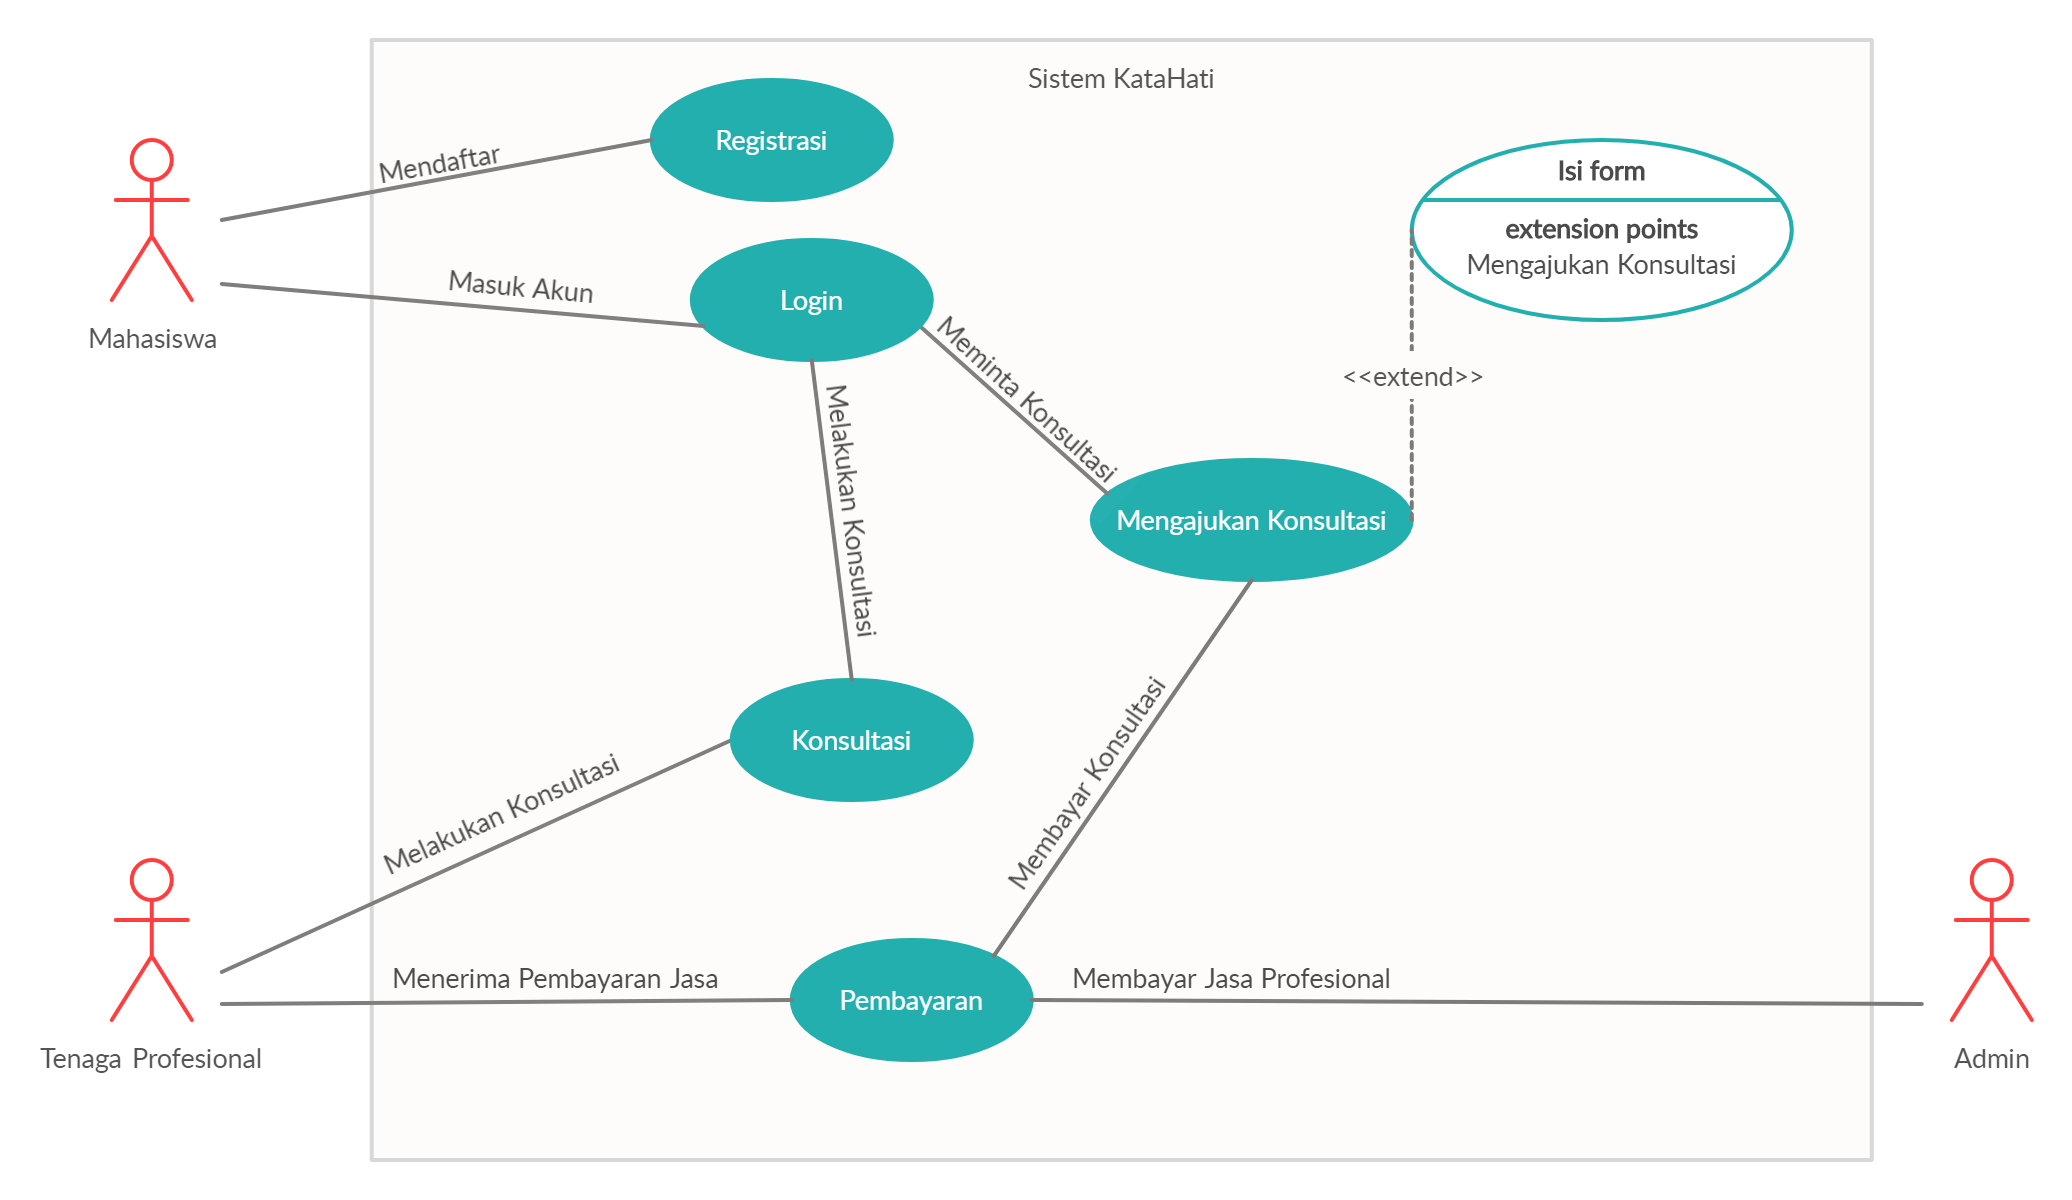
\includegraphics[width=400px]{Use Case Kata Hati.png}
	\end{figure}

	\subsection{Class Diagram}
	\begin{figure}[H]
		\centering
		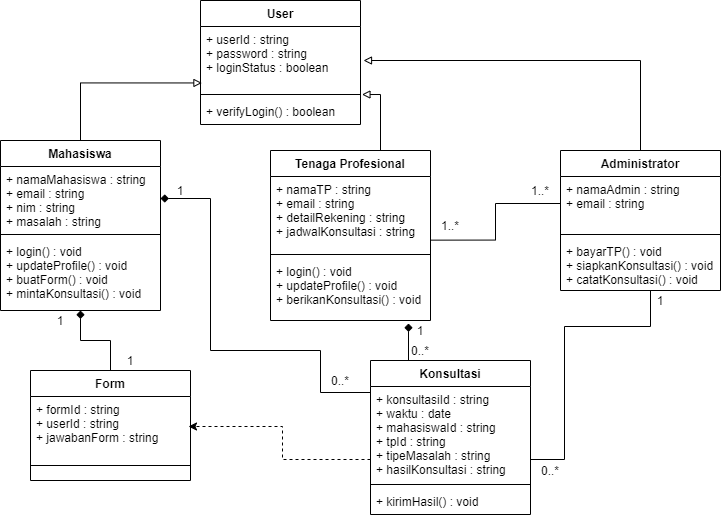
\includegraphics[width=400px]{class_diagram.png}
	\end{figure}

	\subsection{Activity Diagram}
	\begin{figure}[H]
		\centering
		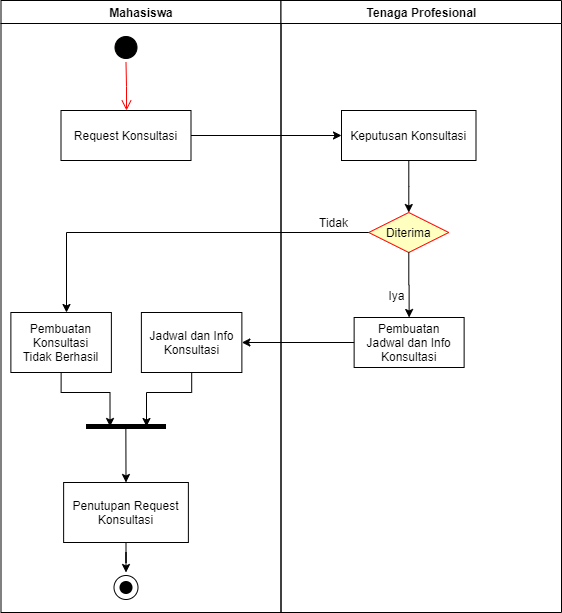
\includegraphics[width=300px]{Activity Diagram.png}
	\end{figure}

	\subsection{Sequential Diagram}
	\subsubsection{Sign Up}
	\begin{figure}[H]
		\centering
		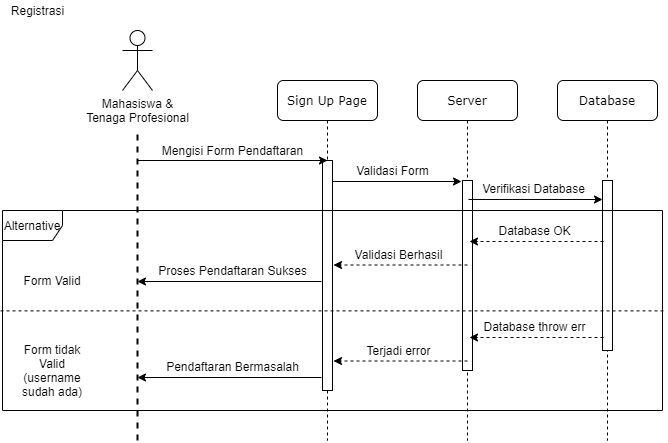
\includegraphics[width=400px]{seq Sign Up.png}
	\end{figure}

	\subsubsection{Pengajuan Konsultasi}
	\begin{figure}[H]
		\centering
		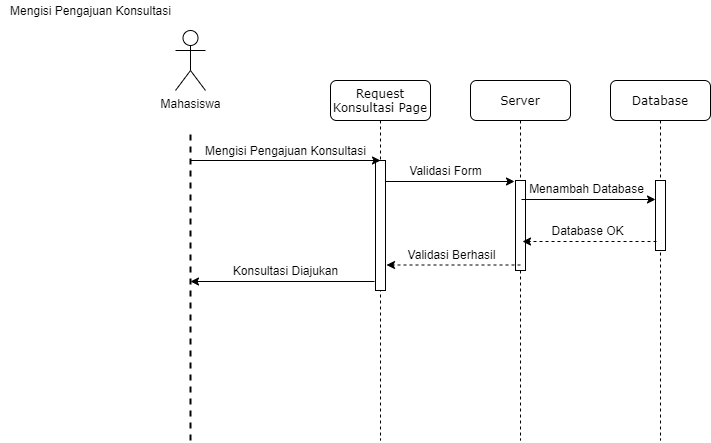
\includegraphics[width=400px]{seq Mengajukan Konsultasi.png}
	\end{figure}

	\subsubsection{Menerima Konsultasi}
	\begin{figure}[H]
		\centering
		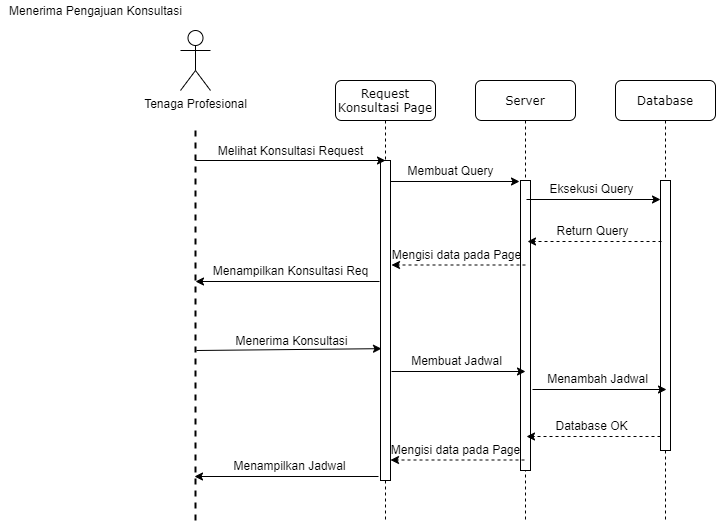
\includegraphics[width=400px]{seq Menerima Konsultasi (1).png}
	\end{figure}

	\section{Screenshot}
	\href{http://yapayapahuy.blitzcorp.cyou/}{YapaYapaHuy.blitzcorp.cyou (*fase percobaan)}
	\subsection{Sudut Pandang Mahasiswa}
	\subsubsection{Home Page}
	\begin{figure}[H]
		\centering
		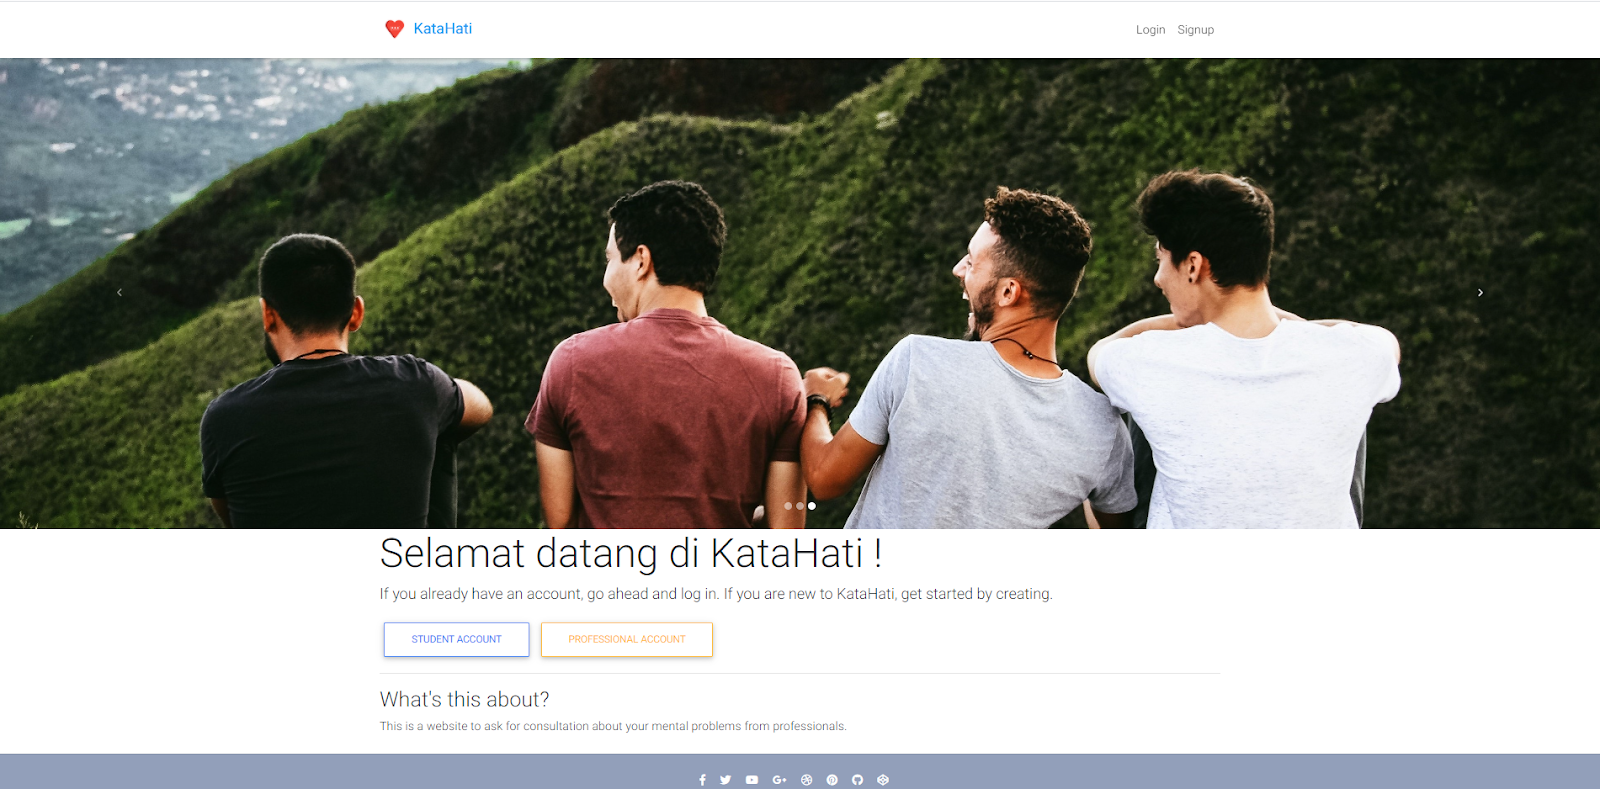
\includegraphics[width=480px]{Home Page.png}
	\end{figure}

	\subsubsection{Sign Up Mahasiswa}
	\begin{figure}[H]
		\centering
		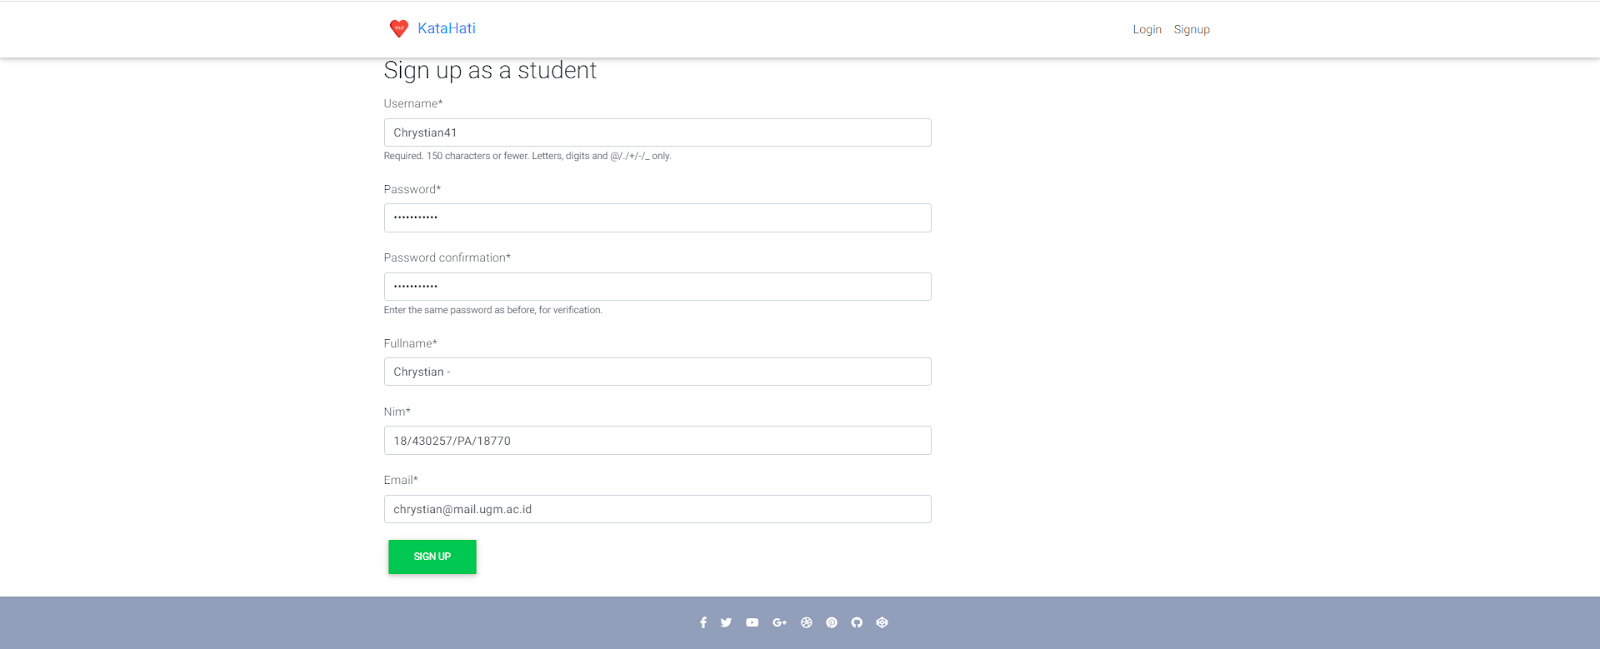
\includegraphics[width=480px]{Sign Up Mahasiswa.png}
	\end{figure}

	\subsubsection{Sign In}
	\begin{figure}[H]
		\centering
		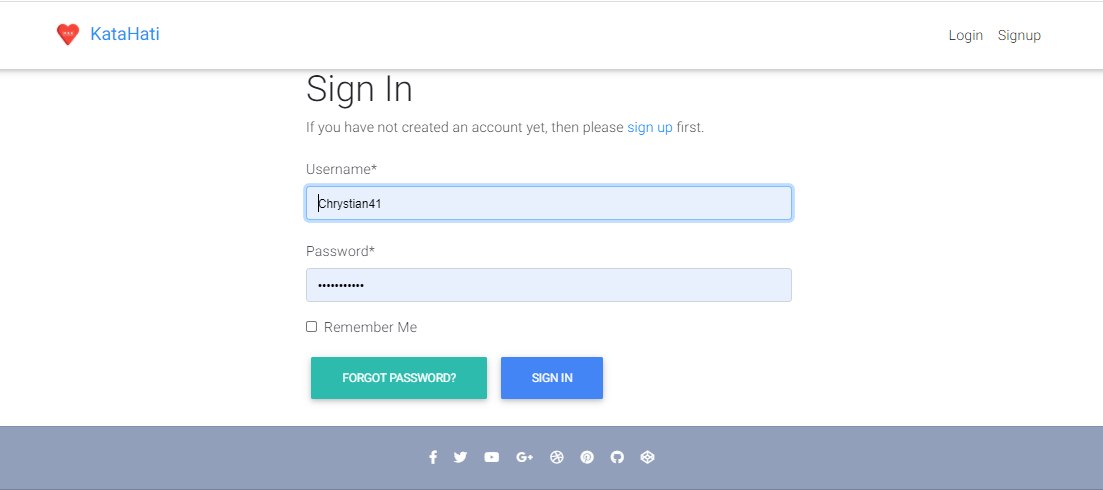
\includegraphics[width=480px]{Sign In.png}
	\end{figure}

	\subsubsection{Student Dashboard}
	\begin{figure}[H]
		\centering
		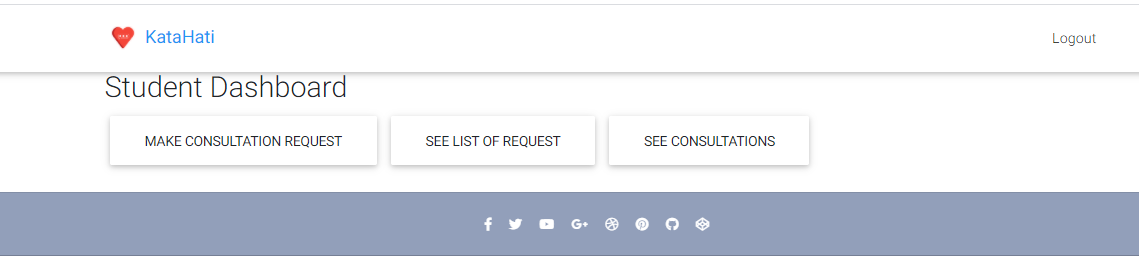
\includegraphics[width=480px]{Student Dashboard.png}
	\end{figure}

	\subsubsection{Make Consultation Request}
	\begin{figure}[H]
		\centering
		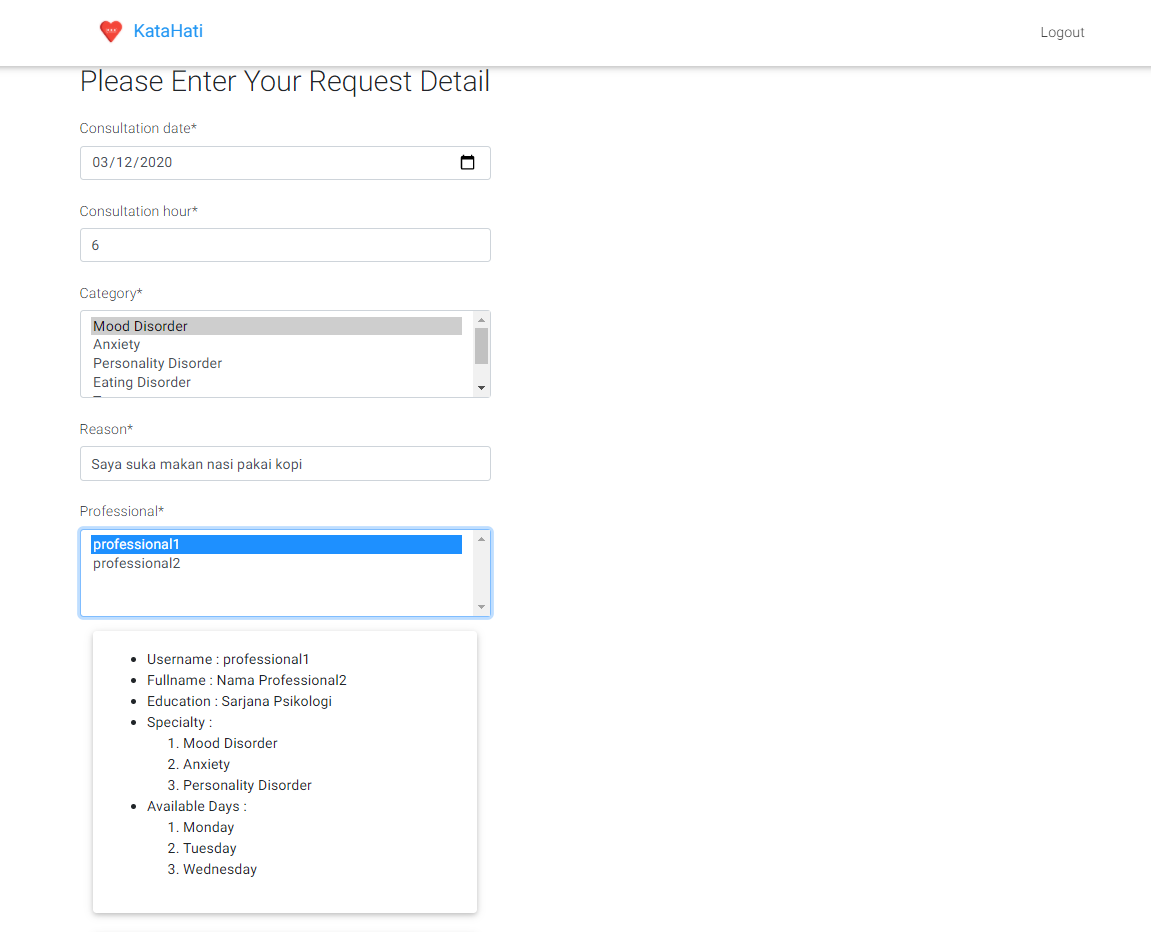
\includegraphics[width=480px]{Consultation Request.png}
	\end{figure}

	\subsubsection{List of Request}
	\begin{figure}[H]
		\centering
		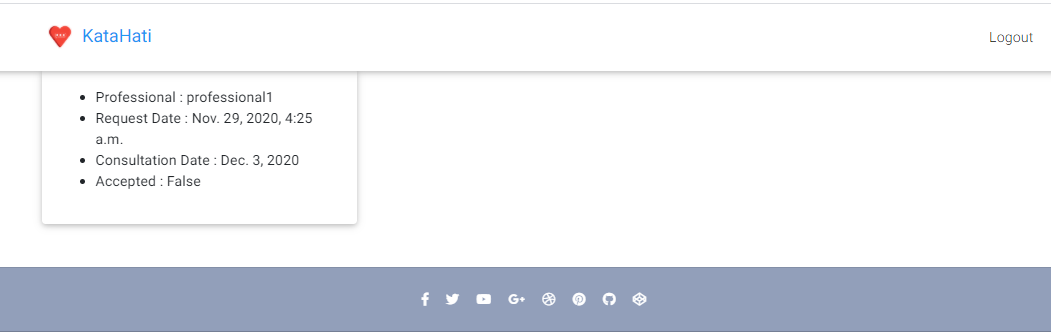
\includegraphics[width=480px]{Request List.png}
	\end{figure}

	\subsubsection{List of Consultation (Diterima)}
	\begin{figure}[H]
		\centering
		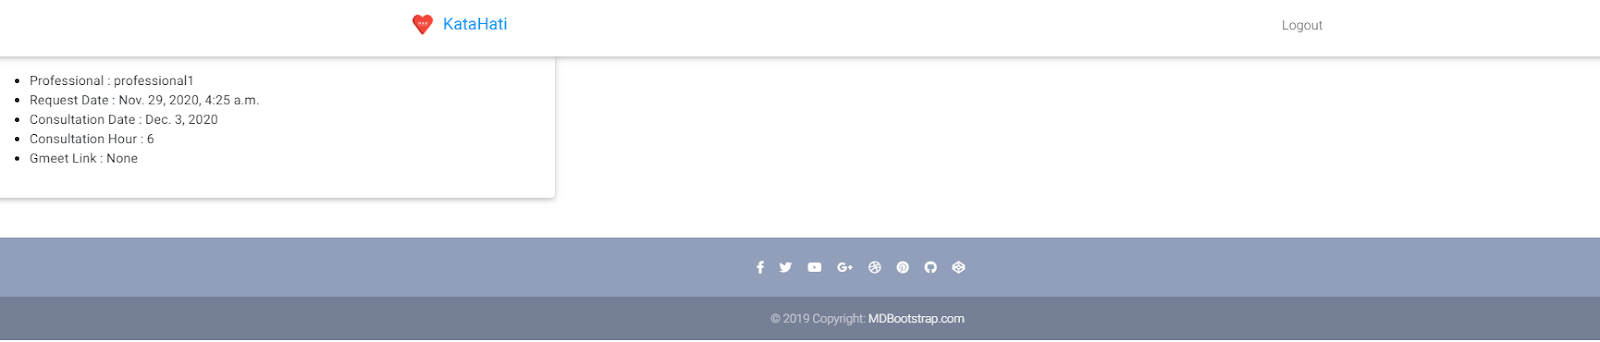
\includegraphics[width=480px]{Consultation.png}
	\end{figure}

	\subsection{Sudut Pandang Professional}
	\subsubsection{Sign In Professional}
	\begin{figure}[H]
		\centering
		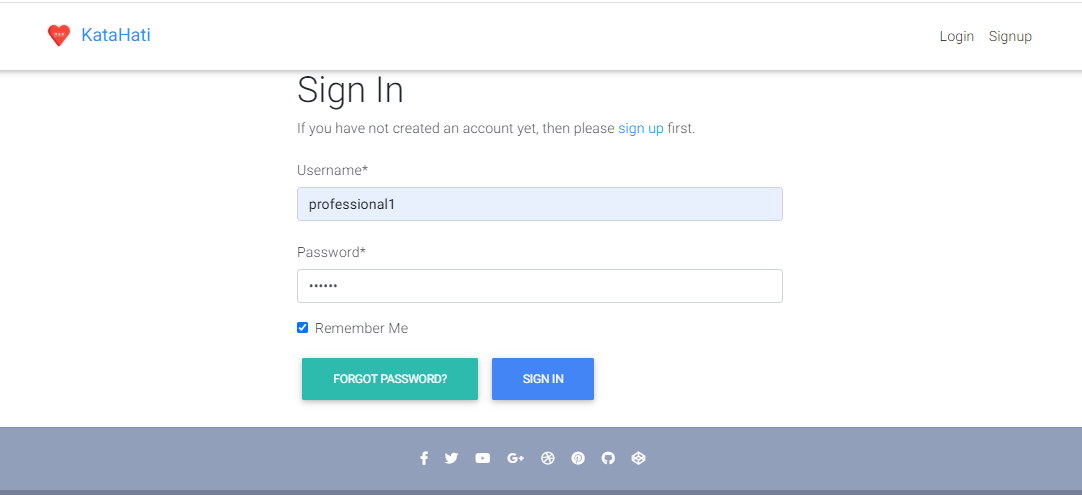
\includegraphics[width=480px]{Sign In Prof.png}
	\end{figure}

	\subsubsection{Professional Dashboard}
	\begin{figure}[H]
		\centering
		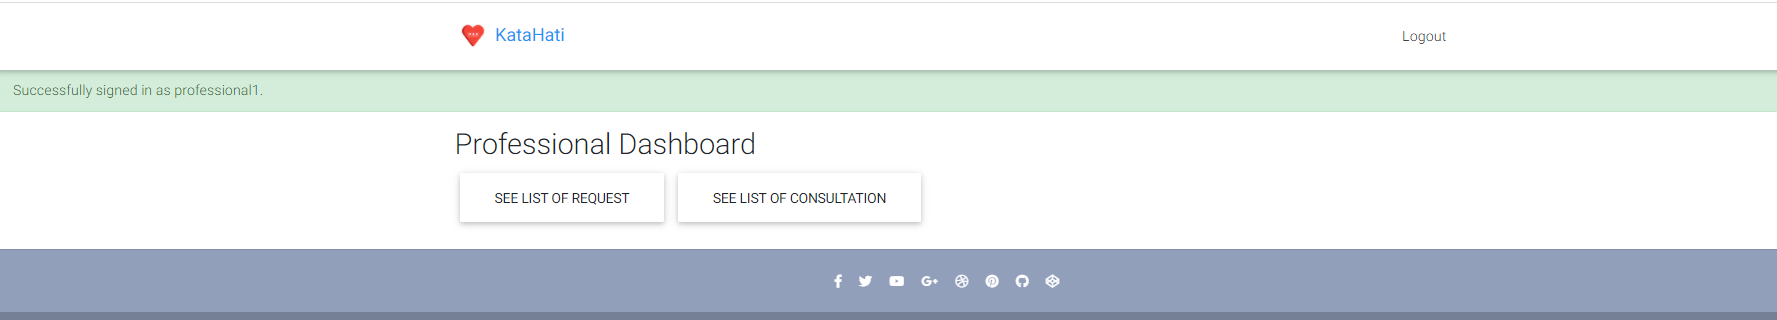
\includegraphics[width=480px]{Prof Dash.png}
	\end{figure}

	\subsubsection{Professional List of Request}
	\begin{figure}[H]
		\centering
		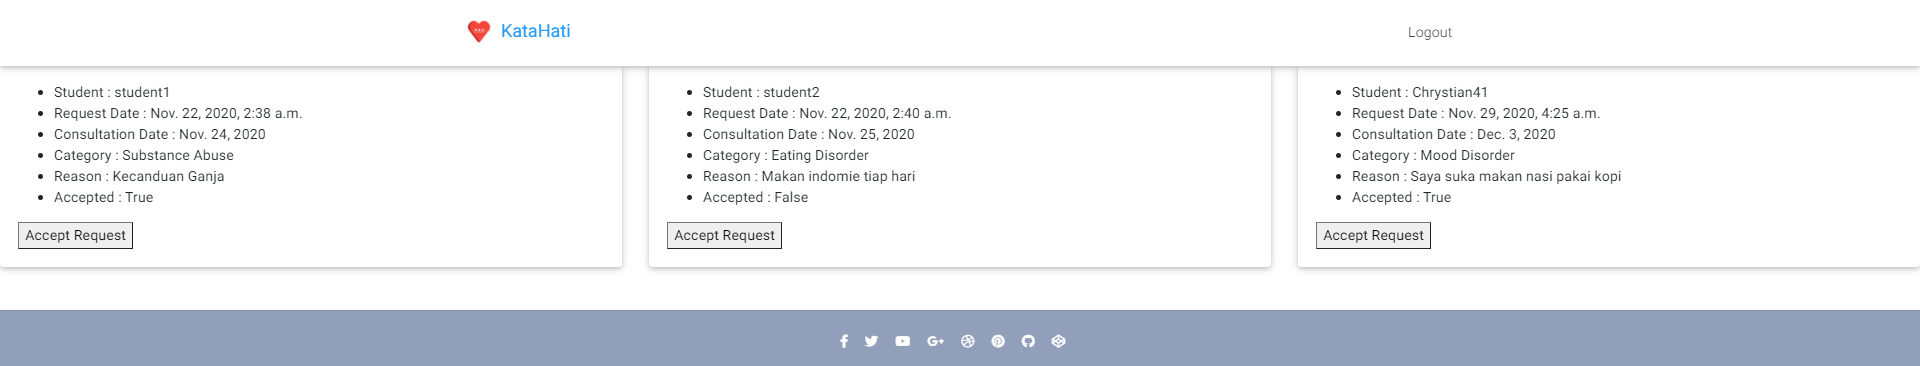
\includegraphics[width=480px]{Prof List.png}
	\end{figure}

	\subsubsection{Professional List of Consultation}
	\begin{figure}[H]
		\centering
		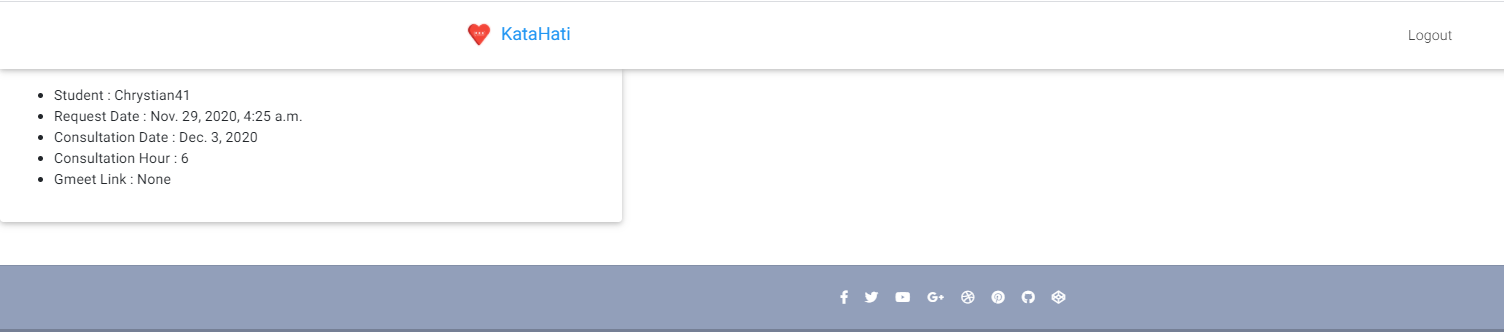
\includegraphics[width=480px]{Prof Active List.png}
	\end{figure}

	\section{Listing Code}
	Seluruh Source Code HTML, CSS, dll. dapat dilihat pada \href{https://github.com/YapaYapaHuy/Final-Project-PPPL}{Link github.com/YapaYapaHuy/Final-Project-PPPL}
	\\
	Beberapa Contoh dari Source Code :
	\subsection{Django urls}
	\begin{verbatim}
from django.urls import path, include

from .views import (
    HomeView,
    StudentFormView,
    ProfessionalFormView,
    StudentDashboardView,
    ProfessionalDashboardView,
    ConsultationRequestView,
)

app_name = 'core'

urlpatterns = [
    path('', HomeView.as_view(), name='home'),
    path('dashboard/student/', StudentDashboardView.as_view(), name="student_dashboard"),
    path('dashboard/professional/', ProfessionalDashboardView.as_view(), name="professional_dashboard"),
]   
	\end{verbatim}

	\newpage
	\subsection{Django Database Model}
	\begin{verbatim}
from django.contrib.auth.models import AbstractUser
from django.db import models
from django.conf import settings

class User(AbstractUser):
	is_student = models.BooleanField(default=False)
	is_professional = models.BooleanField(default=False)

class StudentProfile(models.Model):
	user = models.OneToOneField(
		User, on_delete=models.CASCADE, primary_key=True)
	fullname = models.TextField(default="NAME")
	nim = models.TextField()
	email = models.EmailField(default="EMAIL")

	def __str__(self):
		return self.user.username

class CategoryChoices(models.Model):
	category = models.CharField(max_length=50)

	def __str__(self):
		return self.category

class AvailableDays(models.Model):
	days = models.CharField( max_length=20)

	def __str__(self):
		return self.days

class ProfessionalProfile(models.Model):
	user = models.OneToOneField(
		User, on_delete=models.CASCADE, primary_key=True)
	fullname = models.TextField(null=True)
	email = models.EmailField(null=True)
	education = models.TextField()
	speciality = models.ManyToManyField(CategoryChoices)
	available_days = models.ManyToManyField(AvailableDays)

	def __str__(self):
		return self.user.username

class ConsultationRequest(models.Model):
	# user = models.ForeignKey(
	#     "User", on_delete=models.CASCADE
	# )
	student = models.ForeignKey(
		"StudentProfile",  on_delete=models.SET_NULL, blank=True, null=True
	)
	professional = models.ForeignKey(
		"ProfessionalProfile",  on_delete=models.SET_NULL, blank=True, null=True
	)
	accepted = models.BooleanField(default=False)
	request_date = models.DateTimeField(auto_now_add=True)
	consultation_date = models.DateField(null=True)
	consultation_hour = models.CharField(null=True, max_length=20)
	category = models.ManyToManyField(CategoryChoices)
	reason = models.TextField()
	
	def __str__(self):
		return self.student.user.username

class Consultation(models.Model):
	request = models.ForeignKey(
		"ConsultationRequest", related_name="request", on_delete=models.SET_NULL, blank=True, null=True
	)
	student = models.ForeignKey(
		"StudentProfile", related_name="student", on_delete=models.SET_NULL, blank=True, null=True
	)
	professional = models.ForeignKey(
		"ProfessionalProfile", related_name="professional", on_delete=models.SET_NULL, blank=True, null=True
	)
	gmeet_link = models.TextField(null=True)

	def __str__(self):
		return f"{self.pk}"
	\end{verbatim}
	\newpage

	\subsection{Django Views}
	\begin{verbatim}
from django.db.models.expressions import OrderBy
from django.shortcuts import render
from django.http import HttpResponse
from django.views.generic import ListView, DetailView, View, TemplateView, CreateView
from django.shortcuts import redirect
from django.contrib import messages
from django.contrib.auth import login
from django.http import HttpResponseRedirect, JsonResponse
from django.urls import reverse
from django.utils.decorators import method_decorator
from django.contrib.auth.decorators import login_required
from django.views.generic.edit import UpdateView

from .forms import StudentInitialForm, ProfessionalInitialForm, ConsultationRequestForm
from .models import CategoryChoices, StudentProfile, ProfessionalProfile, Consultation, ConsultationRequest, User

def is_valid_form(values):
	valid = True
	for field in values:
		if field == '':
			valid = False
	return valid

@method_decorator([login_required], name='dispatch')
class DashboardView(View):
	model = User

	def dispatch(self, request, *args, **kwargs):
		if request.user.is_student:
			return redirect("core:student_dashboard")
		elif request.user.is_professional:
			return redirect("core:professional_dashboard")
		return super(DashboardView, self).dispatch(request, *args, **kwargs)

class SignUpView(TemplateView):
	template_name = 'account/signup.html'

class HomeView(TemplateView):
	template_name = "home.html"

class StudentDashboardView(TemplateView):
	template_name = "student_dashboard.html"

class ProfessionalDashboardView(TemplateView):
	template_name = "professional_dashboard.html"

class StudentFormView(CreateView):
	model = User
	form_class = StudentInitialForm
	template_name = "account/signup_form.html"
	
	def get_context_data(self, **kwargs):
		kwargs["user_type"] = "student"
		return super().get_context_data(**kwargs)

	def form_valid(self, form):
		user = form.save()
		login(self.request, user, backend='django.contrib.auth.backends.ModelBackend')
		return redirect("core:student_dashboard")

class ProfessionalFormView(CreateView):
	model = User
	form_class = ProfessionalInitialForm
	template_name = "account/signup_form.html"

	def get_context_data(self, **kwargs):
		kwargs["user_type"] = "professional"
		return super().get_context_data(**kwargs)

	def form_valid(self, form):
		user = form.save()
		login(self.request, user, backend='django.contrib.auth.backends.ModelBackend')
		return redirect("core:professional_dashboard")

class ConsultationRequestView(View):
	
	def get(self, *args, **kwargs):
		form = ConsultationRequestForm()
		context = {
			'form' : form,
			"object_list" : ProfessionalProfile.objects.all()
		}
		return render(self.request, "request_form.html", context)

	def post(self, *args, **kwargs):
		form = ConsultationRequestForm(self.request.POST or None)
		if form.is_valid():
			consultation_date = form.cleaned_data.get("consultation_date")
			consultation_hour = form.cleaned_data.get("consultation_hour")
			category = form.cleaned_data.get("category")[0]
			reason = form.cleaned_data.get("reason")
			professional = form.cleaned_data.get("professional")[0]

			request = ConsultationRequest(
				# user = self.request.user,
				consultation_date = consultation_date,
				consultation_hour = consultation_hour,
				reason = reason,
			)
			request.save()
			category_obj = CategoryChoices.objects.filter(category=category).values_list("id", flat=True)
			request.category.add(category_obj[0])
			request.professional = ProfessionalProfile.objects.filter(user=professional)[0]
			request.student = StudentProfile.objects.filter(user=self.request.user)[0]
			request.save()
		return redirect("dashboard")

class StudentRequestListView(ListView):
	model = ConsultationRequest
	paginate_by = 10
	template_name = "student_request_list.html"

	def get_queryset(self):
		filter_val = StudentProfile.objects.filter(user=self.request.user)[0]
		new_context = ConsultationRequest.objects.filter(
			student=filter_val,
		)
		return new_context

class ProfessionalRequestListView(ListView):
	model = ConsultationRequest
	paginate_by = 10
	template_name = "professional_request_list.html"

	def get_queryset(self):
		filter_val = self.request.user
		new_context = ConsultationRequest.objects.filter(
			professional__user=filter_val,
		)
		return new_context

def ajax_accept_request(request):
	request_id = request.GET.get('request_id')
	consul_request = ConsultationRequest.objects.get(pk=request_id)
	try:
		consul_request.accepted = True
		consul_request.save()
		
		new_consultation = Consultation(
			request = consul_request,
			student = consul_request.student,
			professional = consul_request.professional
			)
		new_consultation.save()

		return JsonResponse({"success": True})
	except Exception as e:
		return JsonResponse({"success": False})

class StudentConsultationListView(ListView):
	model = Consultation
	paginate_by = 10
	template_name = "student_consultation_list.html"

	def get_queryset(self):
		filter_val = StudentProfile.objects.filter(user=self.request.user)[0]
		new_context = Consultation.objects.filter(
			student=filter_val,
		)
		return new_context

class ProfessionalConsultationListView(ListView):
	model = Consultation
	paginate_by = 10
	template_name = "professional_consultation_list.html"

	def get_queryset(self):
		filter_val = ProfessionalProfile.objects.filter(user=self.request.user)[0]
		new_context = Consultation.objects.filter(
			professional=filter_val,
		)
		return new_context
	\end{verbatim}

	\newpage

	\subsection{Django Forms}
	\begin{verbatim}
from django.db.models.fields import CharField
from core.models import AvailableDays, CategoryChoices, ProfessionalProfile, StudentProfile, User, ConsultationRequest, Consultation
from django import forms
from django.contrib.auth.forms import UserCreationForm
from django.db import transaction

class StudentInitialForm(UserCreationForm):
	fullname = forms.CharField(required=True)
	nim = forms.CharField(required=True)
	email = forms.EmailField(required=True)

	class Meta(UserCreationForm.Meta):
		model = User

	@transaction.atomic
	def save(self):
		user = super().save(commit=False)
		user.is_student = True
		user.save()
		student = StudentProfile.objects.create(
			user=user,
			fullname=self.cleaned_data.get('fullname'),
			nim = self.cleaned_data.get('nim'),
			email = self.cleaned_data.get('email'))
		return user

class ProfessionalInitialForm(UserCreationForm):
	fullname = forms.CharField(required=True)
	education = forms.CharField(required=True)
	email = forms.EmailField(required=True)
	speciality = forms.ModelMultipleChoiceField(
		queryset=CategoryChoices.objects.all(),
		widget=forms.CheckboxSelectMultiple,
		required=True)
	available_days = forms.ModelMultipleChoiceField(
		queryset=AvailableDays.objects.all(),
		widget=forms.CheckboxSelectMultiple,
		required=True)  

	class Meta(UserCreationForm.Meta):
		model = User

	@transaction.atomic
	def save(self, commit=True):
		user = super().save(commit=False)
		user.is_professional = True
		user.save()
		professional = ProfessionalProfile.objects.create(
			user=user,
			fullname = self.cleaned_data.get('fullname'),
			education = self.cleaned_data.get('education'),
			email = self.cleaned_data.get('email')
			)
		professional.speciality.add(*self.cleaned_data.get("speciality"))
		professional.available_days.add(*self.cleaned_data.get("available_days"))
		return user

class DateInput(forms.DateInput):
	input_type="date"

class ConsultationRequestForm(forms.Form):

	consultation_date = forms.DateField(widget=DateInput())
	consultation_hour = forms.CharField()
	category = forms.ModelMultipleChoiceField(
		queryset=CategoryChoices.objects.all()
	)
	reason = forms.CharField()
	professional = forms.ModelMultipleChoiceField(
		queryset=ProfessionalProfile.objects.all()
	)
\end{verbatim}

\end{document}